\documentclass[12,]{article}
\usepackage{lmodern}
\usepackage{amssymb,amsmath}
\usepackage{ifxetex,ifluatex}
\usepackage{fixltx2e} % provides \textsubscript
\ifnum 0\ifxetex 1\fi\ifluatex 1\fi=0 % if pdftex
  \usepackage[T1]{fontenc}
  \usepackage[utf8]{inputenc}
\else % if luatex or xelatex
  \ifxetex
    \usepackage{mathspec}
  \else
    \usepackage{fontspec}
  \fi
  \defaultfontfeatures{Ligatures=TeX,Scale=MatchLowercase}
\fi
% use upquote if available, for straight quotes in verbatim environments
\IfFileExists{upquote.sty}{\usepackage{upquote}}{}
% use microtype if available
\IfFileExists{microtype.sty}{%
\usepackage{microtype}
\UseMicrotypeSet[protrusion]{basicmath} % disable protrusion for tt fonts
}{}
\usepackage[margin=1in]{geometry}
\usepackage{hyperref}
\hypersetup{unicode=true,
            pdftitle={Programmieren mit R: Seminararbeit\_1},
            pdfauthor={Daniyar Akhmetov; Marcelo Rainho Avila; Xuan Son Le},
            pdfborder={0 0 0},
            breaklinks=true}
\urlstyle{same}  % don't use monospace font for urls
\usepackage{color}
\usepackage{fancyvrb}
\newcommand{\VerbBar}{|}
\newcommand{\VERB}{\Verb[commandchars=\\\{\}]}
\DefineVerbatimEnvironment{Highlighting}{Verbatim}{commandchars=\\\{\}}
% Add ',fontsize=\small' for more characters per line
\usepackage{framed}
\definecolor{shadecolor}{RGB}{248,248,248}
\newenvironment{Shaded}{\begin{snugshade}}{\end{snugshade}}
\newcommand{\KeywordTok}[1]{\textcolor[rgb]{0.13,0.29,0.53}{\textbf{{#1}}}}
\newcommand{\DataTypeTok}[1]{\textcolor[rgb]{0.13,0.29,0.53}{{#1}}}
\newcommand{\DecValTok}[1]{\textcolor[rgb]{0.00,0.00,0.81}{{#1}}}
\newcommand{\BaseNTok}[1]{\textcolor[rgb]{0.00,0.00,0.81}{{#1}}}
\newcommand{\FloatTok}[1]{\textcolor[rgb]{0.00,0.00,0.81}{{#1}}}
\newcommand{\ConstantTok}[1]{\textcolor[rgb]{0.00,0.00,0.00}{{#1}}}
\newcommand{\CharTok}[1]{\textcolor[rgb]{0.31,0.60,0.02}{{#1}}}
\newcommand{\SpecialCharTok}[1]{\textcolor[rgb]{0.00,0.00,0.00}{{#1}}}
\newcommand{\StringTok}[1]{\textcolor[rgb]{0.31,0.60,0.02}{{#1}}}
\newcommand{\VerbatimStringTok}[1]{\textcolor[rgb]{0.31,0.60,0.02}{{#1}}}
\newcommand{\SpecialStringTok}[1]{\textcolor[rgb]{0.31,0.60,0.02}{{#1}}}
\newcommand{\ImportTok}[1]{{#1}}
\newcommand{\CommentTok}[1]{\textcolor[rgb]{0.56,0.35,0.01}{\textit{{#1}}}}
\newcommand{\DocumentationTok}[1]{\textcolor[rgb]{0.56,0.35,0.01}{\textbf{\textit{{#1}}}}}
\newcommand{\AnnotationTok}[1]{\textcolor[rgb]{0.56,0.35,0.01}{\textbf{\textit{{#1}}}}}
\newcommand{\CommentVarTok}[1]{\textcolor[rgb]{0.56,0.35,0.01}{\textbf{\textit{{#1}}}}}
\newcommand{\OtherTok}[1]{\textcolor[rgb]{0.56,0.35,0.01}{{#1}}}
\newcommand{\FunctionTok}[1]{\textcolor[rgb]{0.00,0.00,0.00}{{#1}}}
\newcommand{\VariableTok}[1]{\textcolor[rgb]{0.00,0.00,0.00}{{#1}}}
\newcommand{\ControlFlowTok}[1]{\textcolor[rgb]{0.13,0.29,0.53}{\textbf{{#1}}}}
\newcommand{\OperatorTok}[1]{\textcolor[rgb]{0.81,0.36,0.00}{\textbf{{#1}}}}
\newcommand{\BuiltInTok}[1]{{#1}}
\newcommand{\ExtensionTok}[1]{{#1}}
\newcommand{\PreprocessorTok}[1]{\textcolor[rgb]{0.56,0.35,0.01}{\textit{{#1}}}}
\newcommand{\AttributeTok}[1]{\textcolor[rgb]{0.77,0.63,0.00}{{#1}}}
\newcommand{\RegionMarkerTok}[1]{{#1}}
\newcommand{\InformationTok}[1]{\textcolor[rgb]{0.56,0.35,0.01}{\textbf{\textit{{#1}}}}}
\newcommand{\WarningTok}[1]{\textcolor[rgb]{0.56,0.35,0.01}{\textbf{\textit{{#1}}}}}
\newcommand{\AlertTok}[1]{\textcolor[rgb]{0.94,0.16,0.16}{{#1}}}
\newcommand{\ErrorTok}[1]{\textcolor[rgb]{0.64,0.00,0.00}{\textbf{{#1}}}}
\newcommand{\NormalTok}[1]{{#1}}
\usepackage{longtable,booktabs}
\usepackage{graphicx,grffile}
\makeatletter
\def\maxwidth{\ifdim\Gin@nat@width>\linewidth\linewidth\else\Gin@nat@width\fi}
\def\maxheight{\ifdim\Gin@nat@height>\textheight\textheight\else\Gin@nat@height\fi}
\makeatother
% Scale images if necessary, so that they will not overflow the page
% margins by default, and it is still possible to overwrite the defaults
% using explicit options in \includegraphics[width, height, ...]{}
\setkeys{Gin}{width=\maxwidth,height=\maxheight,keepaspectratio}
\IfFileExists{parskip.sty}{%
\usepackage{parskip}
}{% else
\setlength{\parindent}{0pt}
\setlength{\parskip}{6pt plus 2pt minus 1pt}
}
\setlength{\emergencystretch}{3em}  % prevent overfull lines
\providecommand{\tightlist}{%
  \setlength{\itemsep}{0pt}\setlength{\parskip}{0pt}}
\setcounter{secnumdepth}{5}
% Redefines (sub)paragraphs to behave more like sections
\ifx\paragraph\undefined\else
\let\oldparagraph\paragraph
\renewcommand{\paragraph}[1]{\oldparagraph{#1}\mbox{}}
\fi
\ifx\subparagraph\undefined\else
\let\oldsubparagraph\subparagraph
\renewcommand{\subparagraph}[1]{\oldsubparagraph{#1}\mbox{}}
\fi

%%% Use protect on footnotes to avoid problems with footnotes in titles
\let\rmarkdownfootnote\footnote%
\def\footnote{\protect\rmarkdownfootnote}

%%% Change title format to be more compact
\usepackage{titling}

% Create subtitle command for use in maketitle
\newcommand{\subtitle}[1]{
  \posttitle{
    \begin{center}\large#1\end{center}
    }
}

\setlength{\droptitle}{-2em}
  \title{Programmieren mit R: Seminararbeit\_1}
  \pretitle{\vspace{\droptitle}\centering\huge}
  \posttitle{\par}
  \author{Daniyar Akhmetov \\ Marcelo Rainho Avila \\ Xuan Son Le}
  \preauthor{\centering\large\emph}
  \postauthor{\par}
  \predate{\centering\large\emph}
  \postdate{\par}
  \date{Abgabedatum: 14/11/2017}


\begin{document}
\maketitle

{
\setcounter{tocdepth}{2}
\tableofcontents
}
\section{Part I (3 Points)}\label{part-i-3-points}

\begin{enumerate}
\def\labelenumi{\arabic{enumi}.}
\tightlist
\item
  \emph{What are the atomic vector types in R?} \emph{Explain which
  value they can take and give an example!}
\item
  \emph{What is the difference between generic and atomic vectors?}
\item
  \emph{Explain the following statement:} \emph{A data frame is a list,
  but not every list is a data frame.}
\end{enumerate}

\textbf{Answer:}

\begin{enumerate}
\def\labelenumi{\arabic{enumi}.}
\tightlist
\item
  Atomic vectors are linear vectors (one-dimensional), which consists of
  values of the same type.
\end{enumerate}

\begin{longtable}[]{@{}lll@{}}
\toprule
\textbf{Atomic vectors} & \textbf{Values} &
\textbf{Examples}\tabularnewline
\midrule
\endhead
logical & TRUE/FALSE & c(TRUE,FALSE)\tabularnewline
integer & integer numbers & c(1L, 10L, 100L)\tabularnewline
numeric & real numbers & c(-26, 1.3, -0.25)\tabularnewline
complex & complex numbers a+bi & c(-2+3i, -4i, 0i)\tabularnewline
character & letters or words & c(``Hello'',``R'',``How are
you'')\tabularnewline
raw & raw bytes (as pairs of hex digits) & as.raw(255) =
ff\tabularnewline
\bottomrule
\end{longtable}

\begin{enumerate}
\def\labelenumi{\arabic{enumi}.}
\setcounter{enumi}{1}
\tightlist
\item
  Generic vectors (lists) are also linear vectors (one-dimensional), but
  can contain objects of different types. Example of a list:
\end{enumerate}

\begin{Shaded}
\begin{Highlighting}[]
\NormalTok{x <-}\StringTok{ }\KeywordTok{list}\NormalTok{(}\DecValTok{1}\NormalTok{:}\DecValTok{10}\NormalTok{,}\StringTok{"a"}\NormalTok{, }\KeywordTok{c}\NormalTok{(}\OtherTok{TRUE}\NormalTok{,}\OtherTok{FALSE}\NormalTok{), }\KeywordTok{c}\NormalTok{(}\DecValTok{1} \NormalTok{+}\StringTok{ }\NormalTok{2i,3i))}
\end{Highlighting}
\end{Shaded}

\begin{enumerate}
\def\labelenumi{\arabic{enumi}.}
\setcounter{enumi}{2}
\tightlist
\item
  A data frame is a list of generic vectors of the same length and
  therefore has a two dimensional structure based on rows and columns.
  Example of a data frame:
\end{enumerate}

\begin{Shaded}
\begin{Highlighting}[]
\NormalTok{df <-}\StringTok{ }\KeywordTok{data.frame}\NormalTok{(}\DataTypeTok{Name =} \KeywordTok{c}\NormalTok{(}\StringTok{"M"}\NormalTok{,}\StringTok{"X"}\NormalTok{,}\StringTok{"D"}\NormalTok{), }
                 \DataTypeTok{Country =} \KeywordTok{c}\NormalTok{(}\StringTok{'B'}\NormalTok{,}\StringTok{'V'}\NormalTok{,}\StringTok{'R'}\NormalTok{), }
                 \DataTypeTok{hasGlasses =} \KeywordTok{c}\NormalTok{(}\OtherTok{FALSE}\NormalTok{,}\OtherTok{TRUE}\NormalTok{,}\OtherTok{TRUE}\NormalTok{))}
\NormalTok{df}
\end{Highlighting}
\end{Shaded}

\begin{verbatim}
##   Name Country hasGlasses
## 1    M       B      FALSE
## 2    X       V       TRUE
## 3    D       R       TRUE
\end{verbatim}

Data frame is a list of lists with the same length. Each list from a
data frame represents a column or a row of a data frame. But a list can
not be a data frame because lists are linear vectors in one dimensional
space. That's why we have the statement.

\section{Part II (7 Points)}\label{part-ii-7-points}

\emph{Explain each line of the following code. In addition, discuss what
the output of identical(a, b) will be. Check the help files for the
functions set.seed, identical, rnorm and cumsum.}

\begin{Shaded}
\begin{Highlighting}[]
  \CommentTok{# ensure that results from a random generator are reproducible}
\KeywordTok{set.seed}\NormalTok{(}\DecValTok{1}\NormalTok{)}
  \CommentTok{# generate a vector of normally distributed random numbers}
\NormalTok{largeVector <-}\StringTok{ }\KeywordTok{rnorm}\NormalTok{(}\FloatTok{1e7}\NormalTok{, }\DataTypeTok{mean =} \DecValTok{5}\NormalTok{, }\DataTypeTok{sd =} \DecValTok{10}\NormalTok{) }
  \CommentTok{# define a and b}
\NormalTok{a <-}\StringTok{ }\KeywordTok{cumsum}\NormalTok{(largeVector)[}\DecValTok{1}\NormalTok{:}\DecValTok{100}\NormalTok{] }
\NormalTok{b <-}\StringTok{ }\KeywordTok{cumsum}\NormalTok{(largeVector[}\DecValTok{1}\NormalTok{:}\DecValTok{100}\NormalTok{])}
  \CommentTok{# is a equal to b?}
\KeywordTok{identical}\NormalTok{(a, b) }
\end{Highlighting}
\end{Shaded}

\begin{verbatim}
## [1] TRUE
\end{verbatim}

\textbf{Answer:}

\begin{itemize}
\item
  Because we ran the function set.seed before, the result of randomly
  choosen largeVector is reproducible for a and b. This means we are now
  working with the only one largeVector.
\item
  A \emph{cumulative sum (cumsum)} is a sequence of partial sums of a
  given sequence.\\
  For instance:\\
  cumsum(largeVector)\\
  = cumsum(c(k1,k2,k3,\ldots{},kn))\\
  = k1 k1+k2 k1+k2+k3 \ldots{} k1+k2+k3+..+kn
\item
  In a we firstly have a cumulative sum of largeVector and then take the
  first 100 elements from it:\\
  a = cumsum(largeVector){[}1:100{]}\\
  a = (k1 k1+k2 k1+k2+k3 \ldots{} k1+k2+k3+\ldots{}+kn){[}1:100{]}\\
  a = k1 k1+k2 k1+k2+k3 \ldots{} k1+k2+k3+\ldots{}+k100
\item
  In b we firstly take the first 100 elements from largeVector and then
  calculate the cumulative sum of these 100 elements.\\
  b = cumsum(largeVector{[}1:100{]})\\
  b = cumsum(k1 k2 k3 \ldots{} k100)\\
  b = k1 k1+k2 k1+k2+k3 \ldots{} k1+k2+k3+\ldots{}+k100
\end{itemize}

\emph{system.time returns the time elapsed for the computation. Explain
the differences:}

\textbf{Answer:}

\begin{Shaded}
\begin{Highlighting}[]
\KeywordTok{system.time}\NormalTok{(}\KeywordTok{cumsum}\NormalTok{(largeVector)[}\DecValTok{1}\NormalTok{:}\DecValTok{100}\NormalTok{])}
\end{Highlighting}
\end{Shaded}

\begin{verbatim}
##    user  system elapsed 
##    0.05    0.00    0.05
\end{verbatim}

\begin{Shaded}
\begin{Highlighting}[]
\KeywordTok{system.time}\NormalTok{(}\KeywordTok{cumsum}\NormalTok{(largeVector[}\DecValTok{1}\NormalTok{:}\DecValTok{100}\NormalTok{]))}
\end{Highlighting}
\end{Shaded}

\begin{verbatim}
##    user  system elapsed 
##       0       0       0
\end{verbatim}

\newpage

\section{Part III (20 Points)}\label{part-iii-20-points}

\emph{Conduct a regression analysis and report your findings. The report
should contain the following sections:}

\begin{itemize}
\tightlist
\item
  \emph{data import}
\item
  \emph{descriptive statistics and data validation}
\item
  \emph{identification of relevant regressors}
\item
  \emph{fitting a regression model}
\item
  \emph{discussion of model fit, e.g.~goodness of fit, significance of
  regressors}
\item
  \emph{interpreting the model}
\end{itemize}

\textbf{Answer:}\\
\textbf{Logistic\_Regression\_Titanic:}

\subsection{Data import}\label{data-import}

Firstly we need to import the necessary libraries and dataset.

\begin{Shaded}
\begin{Highlighting}[]
\KeywordTok{library}\NormalTok{(ggplot2)}
\KeywordTok{library}\NormalTok{(gridExtra) }\CommentTok{# install.packages("gridExtra") if needed}

\KeywordTok{load}\NormalTok{(}\DataTypeTok{file =} \StringTok{"./datasets/titanic.Rdata"}\NormalTok{)}
\end{Highlighting}
\end{Shaded}

\subsection{Descriptive statistics and data
validation}\label{descriptive-statistics-and-data-validation}

Let's take a look at the data to get a general overview of it

\begin{Shaded}
\begin{Highlighting}[]
  \CommentTok{# See which variables are given in the data set through a small sample of the dataset}
\KeywordTok{head}\NormalTok{(titanic,}\DecValTok{5}\NormalTok{)}
\end{Highlighting}
\end{Shaded}

\begin{verbatim}
##   pclass survived                            name    sex     age sibsp
## 1    1st        1   Allen, Miss. Elisabeth Walton female 29.0000     0
## 2    1st        1  Allison, Master. Hudson Trevor   male  0.9167     1
## 3    1st        0    Allison, Miss. Helen Loraine female  2.0000     1
## 4    1st        0 Allison, Mr. Hudson Joshua Crei   male 30.0000     1
## 5    1st        0 Allison, Mrs. Hudson J C (Bessi female 25.0000     1
##   parch ticket     fare   cabin    embarked boat body
## 1     0  24160 211.3375      B5 Southampton    2   NA
## 2     2 113781 151.5500 C22 C26 Southampton   11   NA
## 3     2 113781 151.5500 C22 C26 Southampton        NA
## 4     2 113781 151.5500 C22 C26 Southampton       135
## 5     2 113781 151.5500 C22 C26 Southampton        NA
##                         home.dest
## 1                    St Louis, MO
## 2 Montreal, PQ / Chesterville, ON
## 3 Montreal, PQ / Chesterville, ON
## 4 Montreal, PQ / Chesterville, ON
## 5 Montreal, PQ / Chesterville, ON
\end{verbatim}

Let's summarize the variables

\begin{Shaded}
\begin{Highlighting}[]
\KeywordTok{str}\NormalTok{(titanic)}
\end{Highlighting}
\end{Shaded}

\begin{verbatim}
## 'data.frame':    1309 obs. of  14 variables:
##  $ pclass   : Factor w/ 3 levels "1st","2nd","3rd": 1 1 1 1 1 1 1 1 1 1 ...
##  $ survived :Class 'labelled'  atomic [1:1309] 1 1 0 0 0 1 1 0 1 0 ...
##   .. ..- attr(*, "label")= chr "Survived"
##  $ name     :Class 'labelled'  atomic [1:1309] Allen, Miss. Elisabeth Walton Allison, Master. Hudson Trevor Allison, Miss. Helen Loraine Allison, Mr. Hudson Joshua Crei ...
##   .. ..- attr(*, "label")= chr "Name"
##  $ sex      : Factor w/ 2 levels "female","male": 1 2 1 2 1 2 1 2 1 2 ...
##  $ age      :Class 'labelled'  atomic [1:1309] 29 0.917 2 30 25 ...
##   .. ..- attr(*, "units")= chr "Year"
##   .. ..- attr(*, "label")= chr "Age"
##  $ sibsp    :Class 'labelled'  atomic [1:1309] 0 1 1 1 1 0 1 0 2 0 ...
##   .. ..- attr(*, "label")= chr "Number of Siblings/Spouses Aboard"
##  $ parch    :Class 'labelled'  atomic [1:1309] 0 2 2 2 2 0 0 0 0 0 ...
##   .. ..- attr(*, "label")= chr "Number of Parents/Children Aboard"
##  $ ticket   :Class 'labelled'  atomic [1:1309] 24160 113781 113781 113781 ...
##   .. ..- attr(*, "label")= chr "Ticket Number"
##  $ fare     :Class 'labelled'  atomic [1:1309] 211 152 152 152 152 ...
##   .. ..- attr(*, "units")= chr "British Pound (\\243)"
##   .. ..- attr(*, "label")= chr "Passenger Fare"
##  $ cabin    : Factor w/ 187 levels "","A10","A11",..: 45 81 81 81 81 151 147 17 63 1 ...
##  $ embarked : Factor w/ 3 levels "Cherbourg","Queenstown",..: 3 3 3 3 3 3 3 3 3 1 ...
##  $ boat     : Factor w/ 28 levels "","1","10","11",..: 13 4 1 1 1 14 3 1 28 1 ...
##  $ body     :Class 'labelled'  atomic [1:1309] NA NA NA 135 NA NA NA NA NA 22 ...
##   .. ..- attr(*, "label")= chr "Body Identification Number"
##  $ home.dest:Class 'labelled'  atomic [1:1309] St Louis, MO Montreal, PQ / Chesterville, ON Montreal, PQ / Chesterville, ON Montreal, PQ / Chesterville, ON ...
##   .. ..- attr(*, "label")= chr "Home/Destination"
\end{verbatim}

\begin{longtable}[]{@{}lll@{}}
\toprule
\textbf{variable} & \textbf{description} & \textbf{Notes}\tabularnewline
\midrule
\endhead
pclass & Passenger Class & factor with 3 levels\tabularnewline
survived & Survival & labelled vector\tabularnewline
name & Passenger Name & labelled vector\tabularnewline
sex & Passenger Sex & factor with 2 levels\tabularnewline
age & Passenger Age & labelled vector\tabularnewline
sibsp & Number of Siblings/Spouses Aboard & labelled
vector\tabularnewline
parch & Number of Parents/Children Aboard & labelled
vector\tabularnewline
ticket & Ticket Number & labelled vector\tabularnewline
fare & Passenger Fare & labelled vector\tabularnewline
cabin & Cabin & factor with 187 levels\tabularnewline
embarked & Port of Embarkation & factor with 3 levels\tabularnewline
boat & Lifeboat & factor with 28 levels\tabularnewline
body & Body Identification Number & labelled vector\tabularnewline
home.dest & Home/Destination & labelled vector\tabularnewline
\bottomrule
\end{longtable}

Let's output a descriptive statistic of all variables for an overview of
the data

\begin{Shaded}
\begin{Highlighting}[]
\KeywordTok{summary}\NormalTok{(titanic)}
\end{Highlighting}
\end{Shaded}

\begin{verbatim}
##  pclass       survived         name               sex     
##  1st:323   Min.   :0.000   Length:1309        female:466  
##  2nd:277   1st Qu.:0.000   Class :labelled    male  :843  
##  3rd:709   Median :0.000   Mode  :character               
##            Mean   :0.382                                  
##            3rd Qu.:1.000                                  
##            Max.   :1.000                                  
##                                                           
##       age              sibsp            parch          ticket         
##  Min.   : 0.1667   Min.   :0.0000   Min.   :0.000   Length:1309       
##  1st Qu.:21.0000   1st Qu.:0.0000   1st Qu.:0.000   Class :labelled   
##  Median :28.0000   Median :0.0000   Median :0.000   Mode  :character  
##  Mean   :29.8811   Mean   :0.4989   Mean   :0.385                     
##  3rd Qu.:39.0000   3rd Qu.:1.0000   3rd Qu.:0.000                     
##  Max.   :80.0000   Max.   :8.0000   Max.   :9.000                     
##  NA's   :263                                                          
##       fare                     cabin             embarked        boat    
##  Min.   :  0.000                  :1014   Cherbourg  :270          :823  
##  1st Qu.:  7.896   C23 C25 C27    :   6   Queenstown :123   13     : 39  
##  Median : 14.454   B57 B59 B63 B66:   5   Southampton:914   C      : 38  
##  Mean   : 33.295   G6             :   5   NA's       :  2   15     : 37  
##  3rd Qu.: 31.275   B96 B98        :   4                     14     : 33  
##  Max.   :512.329   C22 C26        :   4                     4      : 31  
##  NA's   :1         (Other)        : 271                     (Other):308  
##       body        home.dest        
##  Min.   :  1.0   Length:1309       
##  1st Qu.: 72.0   Class :labelled   
##  Median :155.0   Mode  :character  
##  Mean   :160.8                     
##  3rd Qu.:256.0                     
##  Max.   :328.0                     
##  NA's   :1188
\end{verbatim}

Since data frame aims to describes the survival status of individual
passengers on the Titanic dependent on many different features. Let's
take a look at some useful graphics.

\begin{Shaded}
\begin{Highlighting}[]
  \CommentTok{# Transform some variables, which are given as a vector}
\NormalTok{titanic$survived <-}\StringTok{ }\KeywordTok{factor}\NormalTok{(titanic$survived)}
\NormalTok{titanic$age <-}\StringTok{ }\KeywordTok{as.numeric}\NormalTok{(titanic$age)}
\NormalTok{titanic$fare <-}\StringTok{ }\KeywordTok{as.numeric}\NormalTok{(titanic$fare)}
\NormalTok{titanic$sibsp <-}\StringTok{ }\KeywordTok{as.numeric}\NormalTok{(titanic$sibsp)}
\NormalTok{titanic$parch <-}\StringTok{ }\KeywordTok{as.numeric}\NormalTok{(titanic$parch)}


\KeywordTok{ggplot}\NormalTok{(titanic, }\KeywordTok{aes}\NormalTok{(survived, }\DataTypeTok{fill =} \NormalTok{survived)) +}\StringTok{ }\KeywordTok{geom_bar}\NormalTok{() +}\StringTok{ }
\StringTok{    }\KeywordTok{scale_fill_discrete}\NormalTok{(}\DataTypeTok{breaks =} \KeywordTok{c}\NormalTok{(}\StringTok{"0"}\NormalTok{, }\StringTok{"1"}\NormalTok{),}\DataTypeTok{labels =} \KeywordTok{c}\NormalTok{(}\StringTok{"No"}\NormalTok{, }\StringTok{"Yes"}\NormalTok{)) +}\StringTok{ }
\StringTok{    }\KeywordTok{labs}\NormalTok{(}\DataTypeTok{subtitle =} \StringTok{"Frequency of survival"}\NormalTok{)}
\end{Highlighting}
\end{Shaded}

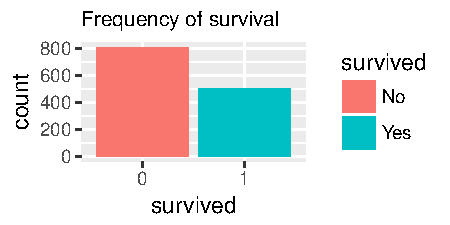
\includegraphics{Seminararbeit_1_files/figure-latex/unnamed-chunk-9-1.pdf}

\begin{Shaded}
\begin{Highlighting}[]
  \CommentTok{# Let's see how survival depends on other variables}
\NormalTok{p1 <-}\StringTok{ }\KeywordTok{ggplot}\NormalTok{(titanic, }\KeywordTok{aes}\NormalTok{(}\DataTypeTok{x =} \NormalTok{sex,}\DataTypeTok{fill =} \NormalTok{survived)) +}\StringTok{ }
\StringTok{    }\KeywordTok{geom_bar}\NormalTok{() +}\StringTok{ }\KeywordTok{scale_fill_discrete}\NormalTok{(}\DataTypeTok{breaks =} \KeywordTok{c}\NormalTok{(}\StringTok{"0"}\NormalTok{, }\StringTok{"1"}\NormalTok{), }\DataTypeTok{labels =} \KeywordTok{c}\NormalTok{(}\StringTok{"No"}\NormalTok{, }\StringTok{"Yes"}\NormalTok{)) +}\StringTok{ }
\StringTok{    }\KeywordTok{labs}\NormalTok{(}\DataTypeTok{subtitle =} \StringTok{"Survival by Sex"}\NormalTok{, }\DataTypeTok{y =} \StringTok{"No. of passengers"}\NormalTok{, }\DataTypeTok{x =} \StringTok{" "}\NormalTok{)}

\NormalTok{p2 <-}\StringTok{ }\KeywordTok{ggplot}\NormalTok{(titanic, }\KeywordTok{aes}\NormalTok{(pclass,}\DataTypeTok{fill =} \NormalTok{survived)) +}\StringTok{ }
\StringTok{    }\KeywordTok{geom_bar}\NormalTok{() +}\StringTok{ }\KeywordTok{scale_fill_discrete}\NormalTok{(}\DataTypeTok{breaks =} \KeywordTok{c}\NormalTok{(}\StringTok{"0"}\NormalTok{, }\StringTok{"1"}\NormalTok{), }\DataTypeTok{labels =} \KeywordTok{c}\NormalTok{(}\StringTok{"No"}\NormalTok{, }\StringTok{"Yes"}\NormalTok{)) +}\StringTok{ }
\StringTok{    }\KeywordTok{labs}\NormalTok{(}\DataTypeTok{subtitle =} \StringTok{"Survival by Passenger class"}\NormalTok{, }\DataTypeTok{y =} \StringTok{"No. of passengers"}\NormalTok{, }\DataTypeTok{x =} \StringTok{" "}\NormalTok{) +}\StringTok{ }
\StringTok{    }\KeywordTok{ylim}\NormalTok{(}\DecValTok{0}\NormalTok{,}\DecValTok{800}\NormalTok{)}
    
\NormalTok{p3 <-}\StringTok{ }\KeywordTok{ggplot}\NormalTok{(titanic, }\KeywordTok{aes}\NormalTok{(sibsp,}\DataTypeTok{fill =} \NormalTok{survived)) +}\StringTok{ }
\StringTok{    }\KeywordTok{geom_bar}\NormalTok{() +}\StringTok{ }\KeywordTok{scale_fill_discrete}\NormalTok{(}\DataTypeTok{breaks =} \KeywordTok{c}\NormalTok{(}\StringTok{"0"}\NormalTok{, }\StringTok{"1"}\NormalTok{), }\DataTypeTok{labels =} \KeywordTok{c}\NormalTok{(}\StringTok{"No"}\NormalTok{, }\StringTok{"Yes"}\NormalTok{)) +}\StringTok{ }
\StringTok{    }\KeywordTok{labs}\NormalTok{(}\DataTypeTok{subtitle =} \StringTok{"Survival by Number of}\CharTok{\textbackslash{}n}\StringTok{Siblings/Spouses Aboard "}\NormalTok{, }
         \DataTypeTok{y =} \StringTok{"No. of passengers"}\NormalTok{, }\DataTypeTok{x =} \StringTok{" "}\NormalTok{)}

\NormalTok{p4 <-}\StringTok{ }\KeywordTok{ggplot}\NormalTok{(titanic, }\KeywordTok{aes}\NormalTok{(parch,}\DataTypeTok{fill =} \NormalTok{survived)) +}\StringTok{ }
\StringTok{    }\KeywordTok{geom_bar}\NormalTok{() +}\StringTok{ }\KeywordTok{scale_fill_discrete}\NormalTok{(}\DataTypeTok{breaks =} \KeywordTok{c}\NormalTok{(}\StringTok{"0"}\NormalTok{, }\StringTok{"1"}\NormalTok{), }\DataTypeTok{labels =} \KeywordTok{c}\NormalTok{(}\StringTok{"No"}\NormalTok{, }\StringTok{"Yes"}\NormalTok{)) +}\StringTok{ }
\StringTok{    }\KeywordTok{labs}\NormalTok{(}\DataTypeTok{subtitle =} \StringTok{"Survival by Number of}\CharTok{\textbackslash{}n}\StringTok{Parents/Children Aboard "}\NormalTok{, }
         \DataTypeTok{y =} \StringTok{"No. of passengers"}\NormalTok{, }\DataTypeTok{x =} \StringTok{" "}\NormalTok{)}

\NormalTok{p5 <-}\StringTok{ }\KeywordTok{ggplot}\NormalTok{(titanic, }\KeywordTok{aes}\NormalTok{(age,}\DataTypeTok{fill =} \NormalTok{survived)) +}\StringTok{ }\KeywordTok{geom_histogram}\NormalTok{(}\DataTypeTok{bins =} \DecValTok{10}\NormalTok{) +}
\StringTok{    }\KeywordTok{scale_fill_discrete}\NormalTok{(}\DataTypeTok{breaks =} \KeywordTok{c}\NormalTok{(}\StringTok{"0"}\NormalTok{, }\StringTok{"1"}\NormalTok{), }\DataTypeTok{labels =} \KeywordTok{c}\NormalTok{(}\StringTok{"No"}\NormalTok{, }\StringTok{"Yes"}\NormalTok{)) +}
\StringTok{    }\KeywordTok{labs}\NormalTok{(}\DataTypeTok{subtitle =} \StringTok{"Survival by Age"}\NormalTok{, }\DataTypeTok{y =} \StringTok{"No. of passengers"}\NormalTok{, }\DataTypeTok{x =} \StringTok{" "}\NormalTok{)}

\NormalTok{p6 <-}\StringTok{ }\KeywordTok{ggplot}\NormalTok{(titanic, }\KeywordTok{aes}\NormalTok{(fare,}\DataTypeTok{fill =} \NormalTok{survived)) +}\StringTok{ }\KeywordTok{geom_histogram}\NormalTok{(}\DataTypeTok{bins =} \DecValTok{10}\NormalTok{) +}
\StringTok{    }\KeywordTok{scale_fill_discrete}\NormalTok{(}\DataTypeTok{breaks =} \KeywordTok{c}\NormalTok{(}\StringTok{"0"}\NormalTok{, }\StringTok{"1"}\NormalTok{), }\DataTypeTok{labels =} \KeywordTok{c}\NormalTok{(}\StringTok{"No"}\NormalTok{, }\StringTok{"Yes"}\NormalTok{)) +}
\StringTok{    }\KeywordTok{labs}\NormalTok{(}\DataTypeTok{subtitle =} \StringTok{"Survival by Age"}\NormalTok{, }\DataTypeTok{y =} \StringTok{"No. of passengers"}\NormalTok{, }\DataTypeTok{x =} \StringTok{" "}\NormalTok{)}

\KeywordTok{grid.arrange}\NormalTok{(p1,p2,p3,p4,p5,p6,}\DataTypeTok{ncol =} \DecValTok{2}\NormalTok{)}
\end{Highlighting}
\end{Shaded}

\begin{verbatim}
## Warning: Removed 263 rows containing non-finite values (stat_bin).
\end{verbatim}

\begin{verbatim}
## Warning: Removed 1 rows containing non-finite values (stat_bin).
\end{verbatim}

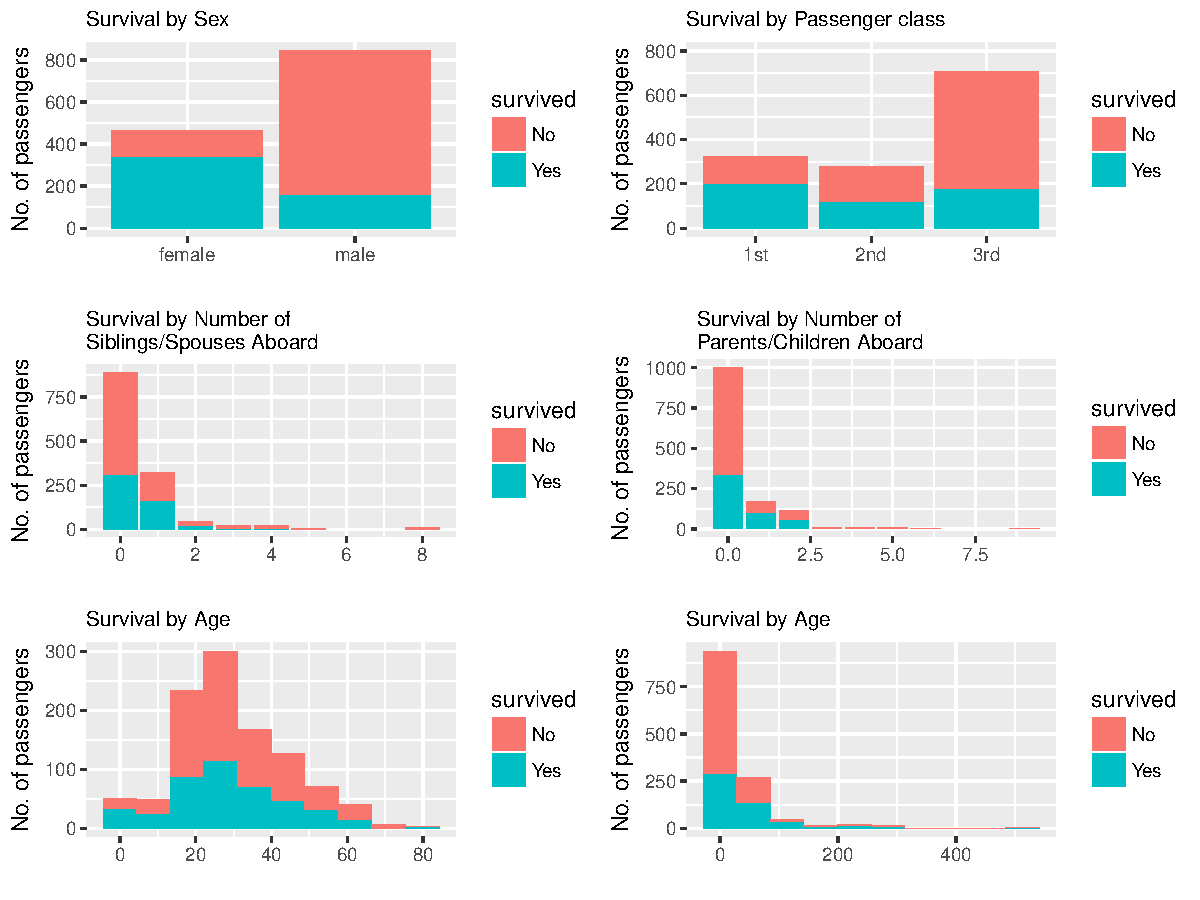
\includegraphics{Seminararbeit_1_files/figure-latex/unnamed-chunk-10-1.pdf}

Let's create some more interesting graphs

\begin{Shaded}
\begin{Highlighting}[]
  \CommentTok{# }
\KeywordTok{ggplot}\NormalTok{(titanic, }\KeywordTok{aes}\NormalTok{(}\DataTypeTok{x =} \KeywordTok{interaction}\NormalTok{(sex,pclass), }\DataTypeTok{fill =} \NormalTok{survived)) +}\StringTok{ }\KeywordTok{geom_bar}\NormalTok{() +}\StringTok{ }
\StringTok{    }\KeywordTok{scale_fill_discrete}\NormalTok{(}\DataTypeTok{breaks =} \KeywordTok{c}\NormalTok{(}\StringTok{"0"}\NormalTok{, }\StringTok{"1"}\NormalTok{), }\DataTypeTok{labels =} \KeywordTok{c}\NormalTok{(}\StringTok{"No"}\NormalTok{, }\StringTok{"Yes"}\NormalTok{))}
\end{Highlighting}
\end{Shaded}

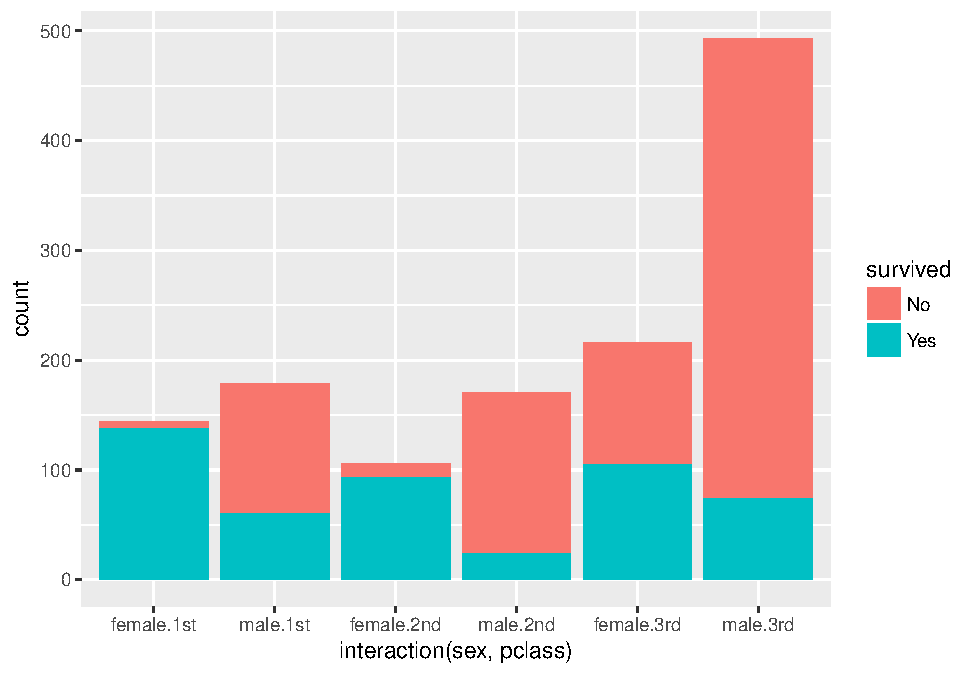
\includegraphics{Seminararbeit_1_files/figure-latex/unnamed-chunk-11-1.pdf}

So after getting the first overlook of our data set as well as the given
variables, let's take a look at possible missing values in the data set

\begin{Shaded}
\begin{Highlighting}[]
\KeywordTok{any}\NormalTok{(}\KeywordTok{is.na}\NormalTok{(titanic))}
\end{Highlighting}
\end{Shaded}

\begin{verbatim}
## [1] TRUE
\end{verbatim}

\begin{Shaded}
\begin{Highlighting}[]
\KeywordTok{sapply}\NormalTok{(titanic, function(x) }\KeywordTok{sum}\NormalTok{(}\KeywordTok{is.na}\NormalTok{(x)))}
\end{Highlighting}
\end{Shaded}

\begin{verbatim}
##    pclass  survived      name       sex       age     sibsp     parch 
##         0         0         0         0       263         0         0 
##    ticket      fare     cabin  embarked      boat      body home.dest 
##         0         1         0         2         0      1188         0
\end{verbatim}

Some first annotations:\\
* The variable \emph{Age} contains about 20\% missing values. We assume
that Age does have influence on predicting the survival, so we will try
to handle these missing values later on.\\
* The varibale \emph{body} contains about 91\% missing values. It is
quite a high amount. Probably we would drop this variable out of our
model.\\
* The amounts of missing vales of \emph{fare} and \emph{embarked} are
very small. Maybe we would just drop the concerned passengers from the
data set or replace the missing values by one certain value.

\subsection{3. Identification of relevant
regressors}\label{identification-of-relevant-regressors}

Let's clean our data due to unnecessary information: Since some
variables do not to contain a lot useful information to our model, we
would drop them from our model. These are: \emph{nam, cabin, ticket,
boat, body, home.dest}

\begin{Shaded}
\begin{Highlighting}[]
\NormalTok{titanic =}\StringTok{ }\NormalTok{titanic[ , !(}\KeywordTok{names}\NormalTok{(titanic) %in%}\StringTok{ }\KeywordTok{c}\NormalTok{(}\StringTok{"name"}\NormalTok{,}\StringTok{"cabin"}\NormalTok{,}\StringTok{"ticket"}\NormalTok{,}\StringTok{"boat"}\NormalTok{,}\StringTok{"body"}\NormalTok{,}\StringTok{"home.dest"}\NormalTok{))]}
\end{Highlighting}
\end{Shaded}

Missing values also need to be handled\\
* Variable \emph{age}: Replace missing values by the mean \emph{age}

\begin{Shaded}
\begin{Highlighting}[]
\NormalTok{titanic$age[}\KeywordTok{is.na}\NormalTok{(titanic$age)] <-}\StringTok{ }\KeywordTok{mean}\NormalTok{(titanic$age,}\DataTypeTok{na.rm =} \OtherTok{TRUE}\NormalTok{)}
\end{Highlighting}
\end{Shaded}

\begin{itemize}
\tightlist
\item
  Variable \emph{fare}: Replace 1 missing value by the mean \emph{fare}
  in the concerned \emph{pclass}.
\end{itemize}

\begin{Shaded}
\begin{Highlighting}[]
\NormalTok{titanic$fare[}\KeywordTok{is.na}\NormalTok{(titanic$fare)] <-}\StringTok{ }\KeywordTok{mean}\NormalTok{(titanic$fare,}\DataTypeTok{na.rm =} \OtherTok{TRUE}\NormalTok{)}
\end{Highlighting}
\end{Shaded}

\begin{itemize}
\tightlist
\item
  Variable \emph{embarked}: Replace 2 missing values by the most
  frequent \emph{embarked} value.
\end{itemize}

\begin{Shaded}
\begin{Highlighting}[]
\KeywordTok{summary}\NormalTok{(titanic$embarked)}
\end{Highlighting}
\end{Shaded}

\begin{verbatim}
##   Cherbourg  Queenstown Southampton        NA's 
##         270         123         914           2
\end{verbatim}

\begin{Shaded}
\begin{Highlighting}[]
\NormalTok{titanic$embarked[}\KeywordTok{is.na}\NormalTok{(titanic$embarked)] <-}\StringTok{ "Southampton"}
\end{Highlighting}
\end{Shaded}

Some variables also need to be relabeled, so that the values (for
example 1,2,3) should not be treated as number but as category.

\begin{Shaded}
\begin{Highlighting}[]
\NormalTok{titanic$pclass <-}\StringTok{ }\KeywordTok{factor}\NormalTok{(titanic$pclass, }
                         \DataTypeTok{levels =} \KeywordTok{c}\NormalTok{(}\StringTok{"1st"}\NormalTok{,}\StringTok{"2nd"}\NormalTok{,}\StringTok{"3rd"}\NormalTok{), }
                         \DataTypeTok{labels =} \KeywordTok{c}\NormalTok{(}\DecValTok{1}\NormalTok{,}\DecValTok{2}\NormalTok{,}\DecValTok{3}\NormalTok{))}
\NormalTok{titanic$sex <-}\StringTok{ }\KeywordTok{factor}\NormalTok{(titanic$sex, }
                      \DataTypeTok{levels =} \KeywordTok{c}\NormalTok{(}\StringTok{"male"}\NormalTok{,}\StringTok{"female"}\NormalTok{), }
                      \DataTypeTok{labels =} \KeywordTok{c}\NormalTok{(}\DecValTok{0}\NormalTok{,}\DecValTok{1}\NormalTok{))}
\NormalTok{titanic$embarked <-}\StringTok{ }\KeywordTok{factor}\NormalTok{(titanic$embarked, }
                           \DataTypeTok{levels =} \KeywordTok{c}\NormalTok{(}\StringTok{"Cherbourg"}\NormalTok{, }\StringTok{"Queenstown"}\NormalTok{, }\StringTok{"Southampton"}\NormalTok{), }
                           \DataTypeTok{labels =} \KeywordTok{c}\NormalTok{(}\DecValTok{1}\NormalTok{, }\DecValTok{2}\NormalTok{, }\DecValTok{3}\NormalTok{)) }
\end{Highlighting}
\end{Shaded}

Before we start modelling, let's check once again, whether all missing
values are handled.

\begin{Shaded}
\begin{Highlighting}[]
\KeywordTok{any}\NormalTok{(}\KeywordTok{is.na}\NormalTok{(titanic))}
\end{Highlighting}
\end{Shaded}

\begin{verbatim}
## [1] FALSE
\end{verbatim}

\textbf{4. Fitting a regression model}\\
Let's create a train and test data set

\begin{Shaded}
\begin{Highlighting}[]
\NormalTok{titanic <-}\StringTok{ }\NormalTok{titanic[}\KeywordTok{sample}\NormalTok{(}\DecValTok{1}\NormalTok{:}\KeywordTok{nrow}\NormalTok{(titanic)),] }\CommentTok{# shuffle the rows}
\NormalTok{train <-}\StringTok{ }\NormalTok{titanic[}\DecValTok{1}\NormalTok{:}\DecValTok{1000}\NormalTok{,] }\CommentTok{# get the first 1000 passengers for training data}
\NormalTok{test <-}\StringTok{ }\NormalTok{titanic[}\DecValTok{1001}\NormalTok{:}\DecValTok{1309}\NormalTok{,] }\CommentTok{# the rest passengers for test data}
\end{Highlighting}
\end{Shaded}

Let's fit the logistic regression model.

\begin{Shaded}
\begin{Highlighting}[]
\NormalTok{model_full <-}\StringTok{ }\KeywordTok{glm}\NormalTok{(survived ~. , }\DataTypeTok{family =} \NormalTok{binomial, }\DataTypeTok{data =} \NormalTok{train) }\CommentTok{# model with all filtered features}
\NormalTok{model_opt <-}\StringTok{ }\KeywordTok{step}\NormalTok{(model_full) }
\end{Highlighting}
\end{Shaded}

\begin{verbatim}
## Start:  AIC=918.48
## survived ~ pclass + sex + age + sibsp + parch + fare + embarked
## 
##            Df Deviance     AIC
## - fare      1   898.51  916.51
## - parch     1   899.43  917.43
## <none>          898.48  918.48
## - sibsp     1   903.94  921.94
## - embarked  2   906.80  922.80
## - age       1   916.39  934.39
## - pclass    2   959.20  975.20
## - sex       1  1158.53 1176.53
## 
## Step:  AIC=916.51
## survived ~ pclass + sex + age + sibsp + parch + embarked
## 
##            Df Deviance     AIC
## - parch     1   899.44  915.44
## <none>          898.51  916.51
## - sibsp     1   903.99  919.99
## - embarked  2   907.27  921.27
## - age       1   916.50  932.50
## - pclass    2   985.55  999.55
## - sex       1  1159.37 1175.37
## 
## Step:  AIC=915.44
## survived ~ pclass + sex + age + sibsp + embarked
## 
##            Df Deviance     AIC
## <none>          899.44  915.44
## - embarked  2   908.14  920.14
## - sibsp     1   906.98  920.98
## - age       1   917.18  931.18
## - pclass    2   987.05  999.05
## - sex       1  1164.94 1178.94
\end{verbatim}

\begin{Shaded}
\begin{Highlighting}[]
\KeywordTok{summary}\NormalTok{(model_opt)}
\end{Highlighting}
\end{Shaded}

\begin{verbatim}
## 
## Call:
## glm(formula = survived ~ pclass + sex + age + sibsp + embarked, 
##     family = binomial, data = train)
## 
## Deviance Residuals: 
##     Min       1Q   Median       3Q      Max  
## -2.4139  -0.6522  -0.4219   0.6240   2.4984  
## 
## Coefficients:
##              Estimate Std. Error z value Pr(>|z|)    
## (Intercept)  1.168909   0.353373   3.308  0.00094 ***
## pclass2     -0.781394   0.254961  -3.065  0.00218 ** 
## pclass3     -2.024333   0.237105  -8.538  < 2e-16 ***
## sex1         2.629094   0.179747  14.627  < 2e-16 ***
## age         -0.029441   0.007137  -4.125 3.71e-05 ***
## sibsp       -0.242525   0.094816  -2.558  0.01053 *  
## embarked2   -0.551085   0.342515  -1.609  0.10763    
## embarked3   -0.639027   0.216451  -2.952  0.00315 ** 
## ---
## Signif. codes:  0 '***' 0.001 '**' 0.01 '*' 0.05 '.' 0.1 ' ' 1
## 
## (Dispersion parameter for binomial family taken to be 1)
## 
##     Null deviance: 1328.13  on 999  degrees of freedom
## Residual deviance:  899.44  on 992  degrees of freedom
## AIC: 915.44
## 
## Number of Fisher Scoring iterations: 5
\end{verbatim}

\textbf{5. Discussion of model fit, e.g.~goodness of fit, significance
of regressors}

\begin{Shaded}
\begin{Highlighting}[]
  \CommentTok{# Predicting the test results}
\NormalTok{test_predict <-}\StringTok{ }\KeywordTok{predict}\NormalTok{(model_opt,}\DataTypeTok{type =} \StringTok{'response'}\NormalTok{,}
                        \DataTypeTok{newdata =} \NormalTok{test[-}\DecValTok{2}\NormalTok{]) }\CommentTok{# apply the model to the test data}
\NormalTok{survived_predict <-}\StringTok{ }\KeywordTok{ifelse}\NormalTok{(test_predict >}\StringTok{ }\FloatTok{0.5}\NormalTok{,}\DecValTok{1}\NormalTok{,}\DecValTok{0}\NormalTok{) }
\NormalTok{confusion_matrix <-}\StringTok{ }\KeywordTok{table}\NormalTok{(test[,}\DecValTok{2}\NormalTok{],survived_predict) }\CommentTok{# create confusion matrix}
\NormalTok{confusion_matrix}
\end{Highlighting}
\end{Shaded}

\begin{verbatim}
##    survived_predict
##       0   1
##   0 157  32
##   1  39  81
\end{verbatim}

\begin{Shaded}
\begin{Highlighting}[]
\NormalTok{accuracy <-}\StringTok{ }\KeywordTok{mean}\NormalTok{(survived_predict ==}\StringTok{ }\NormalTok{test$survived)*}\DecValTok{100}
\KeywordTok{print}\NormalTok{(}\KeywordTok{paste}\NormalTok{(}\StringTok{"Model accuracy is "}\NormalTok{, accuracy, }\StringTok{"%"}\NormalTok{))}
\end{Highlighting}
\end{Shaded}

\begin{verbatim}
## [1] "Model accuracy is  77.0226537216828 %"
\end{verbatim}

\textbf{6. Interpreting the model}

Alternative?:

load(file = ``./datasets/miete.Rdata'')

miete\(bez <- as.integer(miete\)bez)
miete\(wohngut <- factor(miete\)wohngut)
miete\(wohnbest <- factor(miete\)wohnbest)
miete\(ww0 <- factor(miete\)ww0) miete\(zh0 <- factor(miete\)zh0)
miete\(badkach0 <- factor(miete\)badkach0)
miete\(badextra <- factor(miete\)badextra)
miete\(kueche <- factor(miete\)kueche)

Function defines normal/good/best living location myfunction
\textless{}- function(x,y)\{ if (x == `0' \&\& y == `0') \{ return(1) \}
else if (x == 1) \{ return(2) \} else if (y == 1) \{ return(3) \} \}

Apply defined function to wohngut and wohnbest wohnlage \textless{}-
mapply(myfunction, miete\(wohngut, miete\)wohnbest)

Replace variables wohngut and wohnbest by new varibale called wohnlage
miete \textless{}- data.frame(miete{[}1:6{]}, wohnlage, miete{[}9:13{]})

Factorise variable wohnlage: 1 for normal, 2 for good and 3 for best
miete\(wohnlage <- factor(miete\)wohnlage) levels(miete\$wohnlage)
\textless{}- list(normal = 1, gut = 2, best = 3) str(miete)

max\_model \textless{}- lm(formula = nm \textasciitilde{} nmqm + wfl +
rooms + bj + bez + wohnlage + ww0 + zh0 + badkach0 + badextra + kueche,
data = miete) best\_model \textless{}- step(max\_model, direction =
``backward'') max\_model best\_model


\end{document}
